\documentclass[a4paper,oneside,10pt]{article}
\usepackage[utf8]{inputenc}
\usepackage[T1]{fontenc}

\usepackage{makeidx}
\usepackage{graphicx}
\usepackage[french]{babel}
\usepackage{amsmath}
\usepackage{amssymb}
\usepackage{mathrsfs}
\usepackage{lmodern}
\usepackage{listings}
\usepackage{caption}
\usepackage{pgfplots}
\usepackage{hyperref}
\usepackage{url}
\usepackage{csquotes}
\usepackage{mathabx}
\usepackage{fancyhdr}
\pagestyle{fancy}
\fancyhead[L]{\thepage}
\fancyhead[R]{Ensemble Dominant Connexe Glouton}
\cfoot{}

\usepackage{afterpage}
\newcommand\blankpage{%
    \null
    \thispagestyle{empty}%
    \addtocounter{page}{-1}%
    \newpage
}

\pgfplotsset{compat=1.14}

\usepackage{listings}
\usepackage{color}

\definecolor{dkgreen}{rgb}{0,0.6,0}
\definecolor{gray}{rgb}{0.5,0.5,0.5}
\definecolor{mauve}{rgb}{0.58,0,0.82}

\lstset{frame=tb,
  language=Java,
  aboveskip=3mm,
  belowskip=3mm,
  showstringspaces=false,
  columns=flexible,
  basicstyle={\small\ttfamily},
  numbers=none,
  numberstyle=\tiny\color{gray},
  keywordstyle=\color{blue},
  commentstyle=\color{dkgreen},
  stringstyle=\color{mauve},
  breaklines=true,
  breakatwhitespace=true,
  tabsize=3
}

\newtheorem{lemma}{Lemma}

\makeindex
\begin{document}
\title{Algorithme Li et al. : ensemble dominant connexe glouton}
\author{Alexandre Fernandez \& Sylvain Ung}
\maketitle
\thispagestyle{empty}

\hrulefill
\vspace*{1cm}
\begin{center}

\includegraphics[scale=0.15]{images/logo_upmc.jpg}%
\end{center}
\vspace*{1cm}
\hrulefill

\begin{center}\bfseries\Huge
  Rapport de Recherche
\end{center}
\afterpage{\blankpage}

\newpage
\thispagestyle{empty}
\tableofcontents
\newpage
\vspace*{1cm}
\begin{center}\bfseries\Large
Algorithme Li et al. : ensemble dominant connexe glouton
\end{center}

\vspace*{1cm}
\paragraph{}
\textbf{Résumé :} Quelque chose.
\paragraph{}
\textbf{Mots-clés :} Théorie des graphes, ensemble dominant, connexe, NP-complet, algorithme glouton, Li et al.

%\newpage

%\listoffigures
\printindex
%\section{Introduction}
Etant donné un ensemble $\mathcal{S}$ de $n$ points sur $\mathbb R^2$, le rectangle minimum $\mathcal{R}$ est le plus petit rectangle orienté tel que $\forall p \in \mathcal{S}, p \in \mathcal{R}$. Il est évident que l'enveloppe convexe de $\mathcal{S}$ est contenu dans le rectangle minimum, on rappelle que l'enveloppe convexe $\mathcal{E}$ d'un ensemble de points  est le plus petit ensemble convexe qui contient ces points.

Ainsi, l'algorithme de Toussaint pour obtenir le rectangle minimum d'un nuage de points démarre ses calculs à partir d'une enveloppe convexe qu'on aura calculée au préalable. Pour ce faire, il existe plusieurs algorithmes permettant d'obtenir l'enveloppe convexe d'un nuage de points dont les complexités varient selon le cas de figure :
\begin{itemize}
\item Parcours de Graham : $\mathcal{O}(n\log n)$
\item Marche de Jarvis : $\mathcal{O}(nm)$ avec $m$ le nombre de sommets de l'enveloppe convexe ou $\mathcal{O}(n^2)$ dans le pire cas
\item Quickhull : $\mathcal{O}(n\log n)$ ou $\mathcal{O}(n^2)$ dans le pire cas mais en pratique cet algorithme est très efficace et la plus utilisée
\end{itemize}

Dans notre démarche, nous nous servirons du parcours de Graham pour calculer l'enveloppe convexe avant d'appliquer l'algorithme de Toussaint à proprement dit. Dans un deuxième temps, nous renouvellerons l'expérience avec l'algorithme de Ritter calculant le cercle minimum. Les résultats obtenus seront ensuite analysés pour déterminer la qualité en tant que conteneur de ces 2 algorithmes, les détails de l'étude seront montrés dans la partie \ref{efficacite} de ce rapport.

Enfin, nous nous poserons la question de la validité de ces algorithmes sur un espace de dimension 3.
%\newpage
%\section{Algorithmes}
%Nous allons présenter dans cette partie les algorithmes utilisés dans cette étude.
\subsection{Parcours de Graham}
Le parcours de Graham est un algorithme publié par Ronald Graham en 1972 pour calculer l'enveloppe convexe d'un ensemble de points dans un espace de dimension 2 et dont la complexité est en $\mathcal{O}(n)$.

Tout d'abord nous effectuons un pré-calcul afin d'alléger le temps d'exécution de l'algorithme par un filtrage de points dit filtrage par pixel dont le principe est le suivant : étant donné des points ayant la même abscisse, 2 de ces points au plus appartiennent à l'enveloppe convexe. Ainsi, il suffit de ne conserver que les points d'ordonnée maximum et minimum pour chaque ensemble de points ayant la même abscisse. Cette opération en $\mathcal{O}(n)$ réduira la taille de l'entrée de manière significative et ne conservera que les points de l'ensemble les plus pertinents pour le parcours de Graham.

\begin{figure}[ht]
\begin{center}
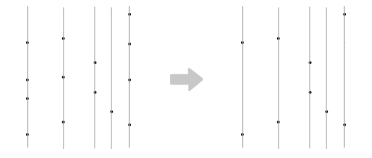
\includegraphics[scale=0.7]{images/tripixel.png}
\caption{Tri pixel}
\end{center}
\end{figure}

Nous allons à présent décrire l'algorithme de Grahamd ont l'idée générale est la suivante : on considère 3 points successifs $P$, $Q$ et $R$ d'abscisse croissant. $Q$ n'appartient à l'enveloppe convexe si et seulement si $R$ est du mauvais côté du demi-plan défini par $PQ$.

\begin{figure}[ht]
\begin{center}
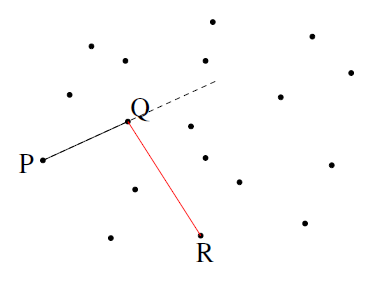
\includegraphics[scale=0.7]{images/graham.png}
\caption{Parcours de Graham}
\end{center}
\end{figure}

On se sert simplement du produit vectoriel afin de déterminer si le triplet \og tourne à droite \fg{} ou \og tourne à gauche \fg{}, on étudie alors le signe du résultat :
\begin{itemize}
\item $0$ : les points sont alignés
\item $>0$ : les points \og tournent à gauche \fg{}
\item $<0$ : les points \og tournent à droite \fg{}
\end{itemize}
En réitérant le processus sur l'ensemble des points on obtient les points constituant l'enveloppe convexe.
%\subsection{Algorithme de Toussaint}
Cet algorithme est basé sur le constat suivant : un des côtés du rectangle minimum doit être colinéaire à l'un des côtés de l'enveloppe convexe. De ce fait, l'algorithme proposé par Godfried Toussaint en 1983 consiste en la recherche de tous les rectangles possibles vérifiant la proposition précédente puis de retenir celui dont l'aire est la plus petite.

Le point délicat de l'implantation de cet algorithme est la bonne gestion de la rotation du rectangle sur les faces de l'enveloppe convexe. Une bonne méthode est de se servir de la technique du \og pied à coulisse \fg{} donnée par Michael Shamos en 1978.

\begin{figure}[ht]
\begin{center}
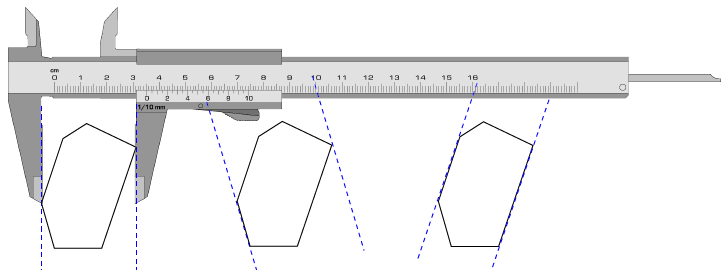
\includegraphics[scale=0.6]{images/shamos.png}
\caption{Technique du pied à coulisse}
\end{center}
\end{figure}

Le point de départ est de construire un rectangle passant par les point cardinaux du plan, autrement dit par les points d'abscisse minimum et maximum ainsi que d'ordonnée maximum et minimum. Cette étape est de complexité linéaire $\mathcal{O}(n)$. On rappelle que l'algorithme de Toussaint implique d'obtenir l'enveloppe convexe au préalable.
A présent, il suffit de nous servir de 2 pieds à coulisse ($NORD-SUD$ et $OUEST-EST$) pour construire les rectangles encadrant notre ensemble de points : puisque le rectangle de départ à été construit à partir des points cardinaux de notre ensemble, tous les points sont nécessairement contenus dans ce rectangle.

Pour savoir de quelle manière est-ce que nous allons faire tourner nos pieds à coulisse il nous faut calculer les angles formés par les côtés du rectangles et les faces de l'enveloppe convexe pour un total de 4 angles $\theta _i$, $\theta _j$, $\theta _k$ et $\theta _l$. A partir de ces angles, nous faisons tourner le rectangle d'un angle $min\{\theta _i, \theta _j, \theta _k, \theta _l\}$.

\newpage
\begin{figure}[ht]
\begin{center}
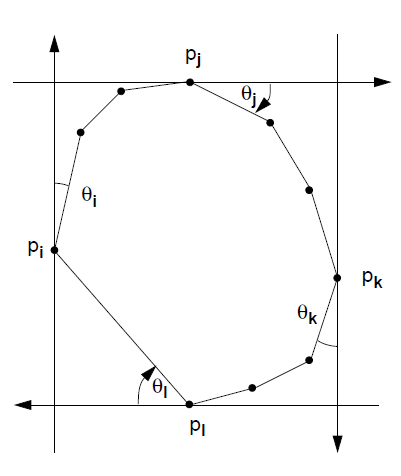
\includegraphics[scale=0.5]{images/toussaint.png}
\caption{Algorithme de Toussaint}
\end{center}
\end{figure}

Une des conditions d'arrêt, plutôt que de traiter toutes les faces possibles de l'enveloppe convexe, serait de s'arrêter lorsque le rectangle aura tourné à plus de $90$\degre ce qui signifierait que nous sommes retombés dans le cas du rectangle initial.

\begin{figure}[ht]
\begin{center}
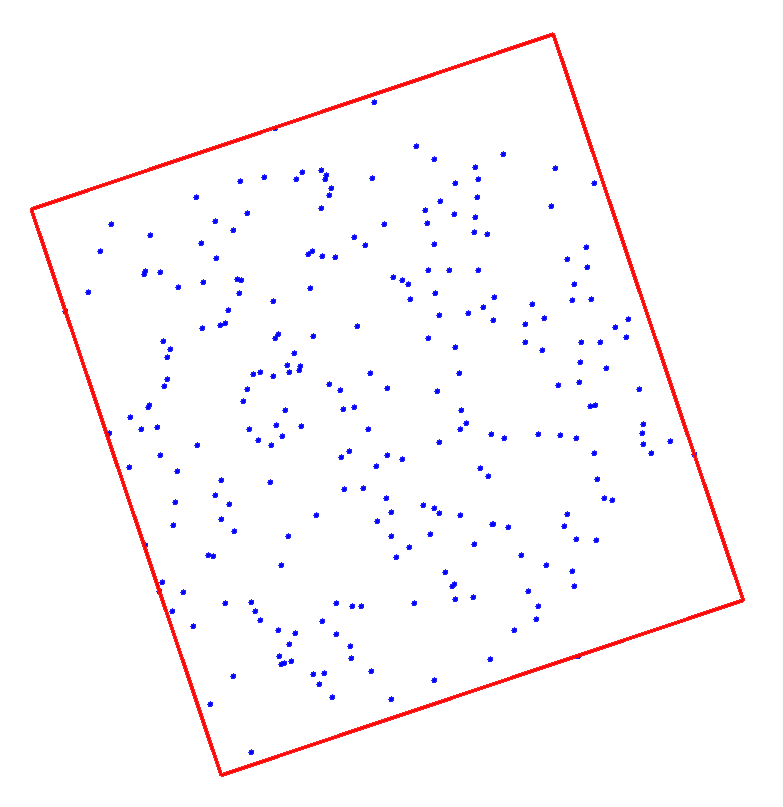
\includegraphics[scale=0.25]{images/ex_toussaint.png}
\caption{Exemple d'application Toussaint}
\end{center}
\end{figure}

Il reste ensuite à calculer l'aire de tous les rectangles obtenus qui peut se faire en temps constant $\mathcal{O}(1)$ (la formule de l'aire d'un polygone convexe peut être utilisée ici et sera décrite dans la partie \ref{efficacite}) pour une complexité totale de $\mathcal{O}(n)$.

Finalement, l'algorithme de Toussaint, bien que les étapes sont au plus de complexité linéaire, est de complexité pseudo-linéaire en $\mathcal{O}(n\log{n})$ car majoré par le calcul de l'enveloppe convexe qui est pseudo-linéaire.
\newpage
%\subsection{Algorithme de Ritter}
Le dernier algorithme utilisé que nous allons présenter et celui de Jack Ritter en 1990 et permet de calculer le cercle minimum. C'est un algorithme glouton, en d'autres mots, l'algorithme retourne une bonne solution mais pas la plus optimale contrairement à un algorithme naïf. En revanche, la perte d'efficacité est gagné en complexité qui s'avère beaucoup plus rapide puisque qu'elle se fait complexité linéaire en la taille de l'entrée $\mathcal{O}(n)$.

\begin{figure}[ht]
\begin{center}
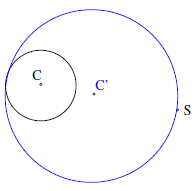
\includegraphics[scale=0.9]{images/ritter.png}
\caption{Algorithme de Ritter}
\end{center}
\end{figure}

L'idée est d'agrandir progressivement le cercle afin de couvrir tous les points de l'ensemble. La description de l'algorithme est donné ci-dessous par  (voir référence \cite{cpa}) :

\begin{enumerate}
\item Prendre un point $dummy$ quelconque appartenant à l'ensemble des points de départ.
\item Parcourir l'ensemble des points pour trouver un point $P$ de distance maximum au point $dummy$.
\item Reparcourir l'ensemble des points pour trouver un point $Q$ de distance maximum au point P.
\item Considérer le point $C$, le centre du segment $PQ$.
\item Considérer le cercle $CERCLE$ centré en $C$, de rayon $\lvert CP \rvert$ : il passe par $P$ et $Q$.
\item Retirer les points $P$ et $Q$ de l'ensemble des points.
\item Tant qu'il reste des points dans l'ensemble, considérer un point $S$ quelconque.
\item Si $S$ est couvert par $CERCLE$, retirer $S$ de l'ensemble des points; répéter l'étape 7.
\item Sinon, tracer au brouillon la droite passant par $S$ et $C$. Celle-ci coupe le périmètre du cercle courant en deux points : soit $T$ le point le plus eloigné de $S$.
\item Déterminer les coordonnées du point $C'$, le centre du segment $ST$.
\item Remplacer $CERCLE$ par le cercle centré en $C$, de rayon $\lvert C'T \rvert$ : il passe par $S$ et $T$.
\item. Repéter 'étape 7. jusqu'à ce qu'il ne reste plus de points dans la liste.
\end{enumerate}

\begin{figure}[ht]
\begin{center}
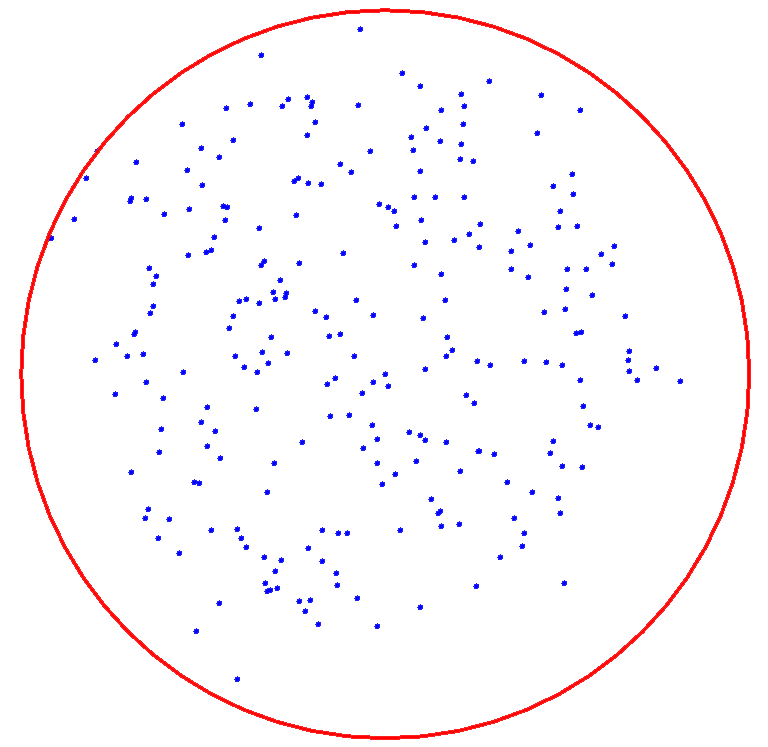
\includegraphics[scale=0.25]{images/ex_ritter.png}
\caption{Exemple d'application Ritter}
\end{center}
\end{figure}
%\newpage
%\section{Mesure des performances}
\label{efficacite}
Dans cette dernière partie nous allons appliquer les différent algorithmes sur un grand nombre d'instances de test contenant chacune 256 points. Cela nous permettra de faire une moyenne sur le temps d'exécution mais aussi sur l'efficacité des conteneurs que sont le rectangle et le cercle par rapport au polygone convexe qui est la plus optimale.

La formule calculant l'efficacité en \%, c'est-à-dire dans quelle proportion est-ce que l'aire du conteneur est plus grand que l'aire de l'enveloppe convexe), est la suivante :
\begin{equation}
\textrm{qualité} = \left( \frac{\textrm{aire}}{\textrm{aire polygone}} \times 100\right) - 100
\end{equation}

Pour calculer l'aire du polygone, nous nous servons de la formule suivante (donnée en \cite{mathwords}) :
\begin{equation}
\textrm{aire polygone} = \frac{1}{2} \begin{vmatrix}
x_1 & y_1 \\
x_2 & y_2 \\
x_3 & y_3 \\
\vdots & \vdots \\
x_n & y_n \\
x_1 & y_1
\end{vmatrix}
\label{aire}
\end{equation}

La formule \eqref{aire} est également utilisée pour calculer l'aire du rectangle. Quand à l'aire du cercle, nous nous servons tout simplement de la formule :
\begin{equation}
\textrm{aire cercle} = \pi r^2
\end{equation}
\subsection{Résultats}
Nous allons ici présenter les résultats obtenus en expérimentant les algorithmes de Toussaint et de Ritter avec 1663 instances de test de la base VAROUMAS fournis. Les algorithmes ont été exécutés sur un ordinateur équipé de 12GB RAM et d'un processeur \textit{Intel Core i7 4790K} cadencé à 4.00GHz tournant sous \textit{Windows 10 Pro 64-bit}.

\begin{center}
\begin{tabular}{|*{4}{c|}}
    \hline
       & Graham  & Toussaint  & Ritter \\
    \hline
     Temps min.  & 0.025103 ms  &0.25538 ms  & 0.009989 ms \\
    \hline
     Temps moy.  & 0.039666 ms  & 0.306384 ms  & 0.019886 ms \\
    \hline
     Temps max.  & 1.697752 ms  & 6.256938 ms & 1.028693 ms \\
    \hline
\end{tabular}
\captionof{table}{Temps d'exécution}
\label{texec}
\end{center}

\begin{figure}[ht]
\begin{center}
\begin{tikzpicture}[font=\small]
    \begin{axis}[
      ybar,
      bar width=30pt,
      ylabel={Temps d'exécution moyen},
      ymin=0,
      ytick=\empty,
      xtick=data,
      axis x line=bottom,
      axis y line=left,
      enlarge x limits=0.2,
      symbolic x coords={Graham, Toussaint,Ritter},
      xticklabel style={anchor=base,yshift=-\baselineskip},
      nodes near coords={\pgfmathprintnumber\pgfplotspointmeta ms}
    ]
      \addplot[fill=white] coordinates {
      	(Graham,0.039666)
        (Toussaint,0.306384)
        (Ritter,0.019886)
      };
    \end{axis}
\end{tikzpicture}
\label{gtime}
\end{center}
\end{figure}

\begin{center}
\begin{tabular}{|*{3}{c|}}
    \hline
       & Toussaint  & Ritter \\
    \hline
     Efficacité  & 25,23\%  & 20,52\%  \\
    \hline
\end{tabular}
\captionof{table}{Efficacité}
\label{eff}
\end{center}

\begin{figure}[ht]
\begin{center}
\begin{tikzpicture}[font=\small]
    \begin{axis}[
      ybar,
      bar width=30pt,
      ylabel={Efficacité},
      ymin=0,
      ytick=\empty,
      xtick=data,
      axis x line=bottom,
      axis y line=left,
      enlarge x limits=0.2,
      symbolic x coords={Toussaint,Ritter},
      xticklabel style={anchor=base,yshift=-\baselineskip},
      nodes near coords={\pgfmathprintnumber\pgfplotspointmeta\%}
    ]
      \addplot[fill=white] coordinates {
        (Toussaint,25.23)
        (Ritter,20.52)
      };
    \end{axis}
\end{tikzpicture}
\label{geff}
\end{center}
\end{figure}
\subsection{Interprétation}
D'après les résultats obtenus, on remarque que l'algorithme de Toussaint prend largement plus de temps à s'exécuter par rapport à l'algorithme de Ritter. En effet, nous avions vu que l'algorithme de Toussaint était pseudo-linéaire, dû au parcours préliminaire de Graham, alors que celui de Ritter est linéaire. Dans un cas défavorable, on peut même observer que l'algorithme de Toussaint est 6 fois plus long en exécution que celui de Ritter.

En terme d'efficacité, l'algorithme de Ritter est également plus optimale puisque que la superficie du cercle minimum est en moyenne 20.52\% plus grand que celle de l'enveloppe convexe, contre 25.35\% pour le rectangle minimum.

On pourrait prendre d'autres critères d'évaluation que le temps d'exécution ou l'efficacité comme la complexité mémoire par exemple, qui serait elle aussi à l'avantage de l'algorithme de Ritter étant donné que celui de Toussaint requiert la conservation en mémoire de beaucoup plus de paramètres.

\paragraph{}
Tout porte à croire que l'algorithme de Ritter est largement préférable à celui de Toussaint, pour en être sûr il aurait fallu expérimenter sur un plus large éventail de test que celui de VAROUMAS et sur des instances plus grandes : 256 points constitue en effet une instance de taille relativement petite.

En revanche, pour en revenir au temps d'exécution, l'algorithme de Toussaint semble être un bon candidat à la parallélisation. En effet, on pourrait répartir les calculs de chaque rectangle et les exécuter en parallèle avant de finalement comparer leur superficie, contrairement à l'algorithme de Ritter qui n'est pas parallélisable puisque c'est un algorithme glouton. Si cette parallélisation s'avère efficace, le temps d'exécution moyen s'en trouverait largement réduit même si le parcours de Graham est toujours présent dont le temps d'exécution est supérieur à Ritter.
%Finalement, il s'avère que l'algorithme de Toussaint est moins efficace que l'algorithme de Ritter, que ce soit en terme de temps d'exécution, d'efficacité en tant que conteneur ou même de complexité mémoire. Cependant, comme dit précédemment, c'est un algorithme qui à l'air de bien se prêter à la parallélisation. Une des raisons qui pourrait pousser à préférer l'algorithme de Toussaint à celui de Ritter serait la volonté d'obtenir un conteneur de forme rectangulaire plutôt que circulaire pour être plus fidèle à un problème posé. En effet, tout dépend de la forme globale de la répartition des points et, plus généralement, du contexte du problème considéré.

Une dernière question que l'on pourrait se poser serait celle de la validité de ces algorithmes en 3 dimensions. Fondamentalement, cela ne change pas grand chose pour l'algorithme de Ritter, l'idée générale reste la même et il suffit d'adapter les formules pour un espace de dimension 3. En revanche, cela risque d'être plus compliqué pour le rectangle qui deviendrait alors un parallélépipède. Joseph O'Rourke a proposé une solution en 1985 dont la complexité est cubique, ce qui est bien supérieur à la complexité pseudo-linéaire de la version 2D. L'idée étant que 2 des 6 faces du parallélépipède doit être coplanaire avec 2 des arêtes de l'enveloppe convexe.
%\newpage
%\nocite{*}
%\bibliographystyle{plain}
%\bibliography{bibliographie/ref}
\end{document}